\documentclass[a4paper, 12pt]{article}
\usepackage[utf8]{inputenc}  % Unicode
\usepackage[french]{babel}
\usepackage{geometry}
\usepackage{graphics}
\usepackage[pdftex]{graphicx, color}
\usepackage{pdfpages}
\DeclareGraphicsExtensions{.jpg,.png}
\pdfoutput=1
\usepackage[pdftex,
	bookmarks = true,           % Signets
	bookmarksnumbered = true,   % Signets numerotes
	pdfstartview = FitV,        % La page prend toute la hauteur
	colorlinks=true,
	citecolor=black,urlcolor=blue,linkcolor=black,
	pdfauthor={Auteur},
	pdftitle={Titre},
 	pdfsubject={Sujet},
%	pdfkeywords={},	% Besoin de keywords ?
	plainpages=false,
	pdfpagelabels,
	breaklinks=true,
   	hyperindex,
	linktocpage=true	% pour colorier seulement le numéros dans la TOC	
]{hyperref}
\usepackage{float}
\usepackage{listings}
\usepackage{alltt}
\usepackage{amsmath}
\renewcommand{\ttdefault}{txtt}

\lstset{basicstyle=\ttfamily,
escapeinside={||},
mathescape=true}
\setcounter{secnumdepth}{3}
\newcommand{\HRule}{\rule{\linewidth}{0.5mm}}

\newcommand*\styleC{\fontsize{9}{10pt}\selectfont }
\newcommand*\styleD{\fontsize{9}{10pt}\usefont{OT1}{pag}{m}{n}\selectfont }

\makeatletter
% on fixe le langage utilisé
\lstset{language=matlab}
\edef\Motscle{emph={\lst@keywords}}
\expandafter\lstset\expandafter{
}
\makeatother



\definecolor{Ggris}{rgb}{0.45,0.48,0.45}

\lstset{emphstyle=\ttfamily\color{blue}, % les mots réservés de matlab en bleu
basicstyle=\ttfamily\styleC, % 
keywordstyle=\ttfamily,
commentstyle=\color{Ggris}\styleD, % \styleD commentaire en gris
numberstyle=\tiny\color{black},
numbers=left,
numbersep=10pt,
lineskip=0.7pt,
showstringspaces=false}
%  % inclure le fichier source
\newcommand{\FSource}[1]{%
\lstinputlisting[texcl=true]{#1}
}

%%%%%%%%%
\textwidth=15cm
\textheight=21cm
%\hoffset=-2.5cm
\tolerance=9000
\hbadness=9000
\pretolerance=2500


\begin{document}
%\rmfamily

\begin{titlepage}
\begin{center}



\textsc{\Large Rapport de TP - SY26}\\[0.5cm]
\vspace{4cm}
% Title
\HRule \\[0.4cm]
{ \huge \bfseries TP02 - Codage de Huffman \\[0.4cm] }

\HRule \\[1.5cm]

% Author and supervisor
\begin{minipage}{0.4\textwidth}
\begin{flushleft} \large
R\'emi \textsc{Burtin}
\end{flushleft}
\end{minipage}
\begin{minipage}{0.4\textwidth}
\begin{flushright} \large
Cyril \textsc{Fougeray}
\end{flushright}
\end{minipage}

\vspace{4cm}

{\large \today}



\vfill
% Bottom

\includegraphics[width=0.25\textwidth]{logo.jpg}\\[0.5cm]

\textsc{\LARGE Universit\'{e} de Technologie de Compi\`{e}gne}\\[1.5cm]


\end{center}
\end{titlepage}


%\begin{abstract} 
%\end{abstract} 

%{\bf Keywords:} \newline


\clearpage

\section{Introduction}

L’objectif de ce TP est la mise en œuvre du codage de canal pour simuler leur capacité de correction et en cerner les limites. Nous allons étudier les codes en bloc (linéaires ou cycliques), pour lesquels des blocs de k symboles d’information sont protégés indépendamment les uns des autres par m symboles de contrôle pour former des mots codes à n symboles.\\


\section{Codage de Hamming}

\subsection{Question 1 - Codage}

Pour calculer un mot code à partir de la matrice de contrôle de parité $\mathbf{H} = [\mathbf{P}^T | \mathbf{I}_{n-k}]$ et d'un bloc d'information $\mathbf{m}$, il nous suffit de calculer la matrice génératrice $\mathbf{G}$ qui est définie par $[\mathbf{I}_k | \mathbf{P}]$. Puis on obtient le mot code $\mathbf{c}$ en multipliant $\mathbf{m}$ et $\mathbf{G}$ (multiplication modulo 2). Voir fonction \textit{hamcode} en annexe \ref{hamcode}. La matrice de contrôle de parité $\mathbf{H}$ est quant à elle calculer via la fonction MATLAB \textit{hammgen}. Cette fonction prend un paramètre $M$ permettant le calcul de la longueur du mot code en suivant la relation $N=2^M-1$. \\

\subsection{Question 2 - Décodage}

Afin de décoder le mot code précédemment créé, éventuellement entaché d'erreurs, nous avons mis en place une fonction \textit{hamdecode} (\textit{cf.} \ref{hamdecode}) prenant en paramètre le mot code et la matrice de contrôle de parité.
Pour cela, nous commençons par calculer le syndrome $s = r\times H^T$ ($r$ étant le mot encodé), permettant de retrouver les éventuelles erreurs glissées dans le mot encodé. En effet, si $s$ est différent de 0, alors il existe une erreur dans le mot encodé. Cette erreur se retrouve facilement une fois la table des syndromes calculée.
Ici, nous ajoutons trois bits de redondance au mot à encoder, il y aura donc $2^3$ syndromes possibles. Pour chacun de ces syndromes, on cherche si il existe une configuration $e$ de 1 erreur, puis de 2 erreurs, puis de 3... telle que $s = e \times H^t$. Pour $s=0$, $e=0$ : il n'existe pas d'erreur. Ainsi, nous pouvons détecter $2^3 - 1 = 7$ erreurs différentes, soit une erreur sur une seule bit du message encodé. Une fonction MATLAB permet de calculer directement la table des syndromes en lui passant la matrice de contrôle de parité : \textit{syndtable}. Sur chaque ligne de la matrice retournée par \textit{syndtable} apparait $e$, correspondant à la position du ou des bits d'erreur. Une opération logique XOR permet donc de corriger l'erreur dans le mot à décoder et de retourner le bon mot code. Nous avons fait le test en insérant une erreur :
\begin{alltt}
>> H = hammgen(3); % creation de la matrice de controle de parite
>> c = hamcode([1 0 1 0], H) % encodage du mot 0101
c =
     0     0     1   |   \textit{1     0     1     0}
		
% decodage avec inclusion d'une erreur
>> cdecode = hamdecode( xor([0 1 0 0 0 0 0], c), H)
cdecode =
     0     0     1   |   \textit{1     0     1     0}
		
% decodage avec inclusion de deux erreurs (limites)
>> cdecode = hamdecode( xor([0 1 0 0 0 0 1], c), H)
cdecode =
     0     \textit{1 }    1     \textit{1}     0     \textit{0     1}
\end{alltt}

Les bits de redondance sont ajoutés au début (trois premiers bits). Nous observons que si un bit contient une erreur, l'erreur est corrigée car le message retourné par le décodage est retrouvé. Par contre, si deux bits du message sont erronés, la table des syndromes ne permet pas de retrouver les erreurs, le message est alors altéré.

\section{Codage BCH}

Pour récupérer le polynôme générateur BCH permettant de corriger 3 erreurs sur 15 bits, on appelle la fonction \textit{bchgenpoly} en lui passant les valeurs de $n$ et $k$, qui sont en l’occurrence 15 et 5. Nous générons ensuite un message aléatoire de longueur $k$ avec la fonction \textit{randi}, que nous mettons sous forme de tableau d’éléments du corps de Galois grâce à la fonction \textit{gf}. \\
Pour coder le message généré, on le passe avec $n$ et $k$ à la fonction \textit{bchenc}. Puis on ajoute 3 erreurs aléatoires :
\begin{alltt}
code_bruite = code + randerr(1,n,3)
\end{alltt}
Une fois le message bruité, on peut effectuer le décodage avec la fonction \textit{bchdec} qui nous renvoie le message décodé ainsi que le nombre d'erreurs corrigées.
Voir code en annexe \ref{bchtest}.

% \section{Codes convolutifs}

% \begin{figure}[H]
% 	\centering
% 	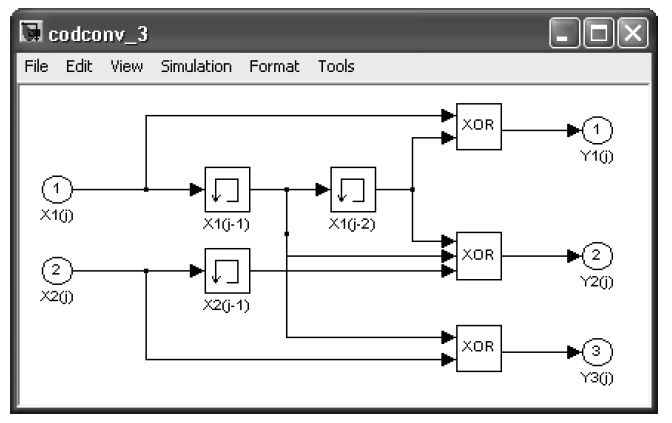
\includegraphics[scale=0.8]{../codeur_convolutif_exo.png}
% 	\caption{Codeur convolutif (3,2,2)}
% 	\label{fig:cod_convolutif}
% \end{figure}

% Les équations des différentes sorties $Y_j$ sont les suivantes :

% \[ Y_j^1 = X_{j}^1 + X_{j-2}^1 \]
% ce qui donne sous la forme matricielle :
% \[ G = \begin{bmatrix} 1 & 0 & 1 \\ 0 & 0 & 0 \end{bmatrix} \] 

% \[ Y_j^2 = X_{j-1}^1 + X_{j-2}^1 + X_{j-1}^2 \]
% ce qui donne sous la forme matricielle :
% \[ G = \begin{bmatrix} 0 & 1 & 0 \\ 0 & 1 & 0 \end{bmatrix} \]

% \[ Y_j^3 =  X_{j-1}^1 + X_{j}^2 \]
% ce qui donne sous la forme matricielle :
% \[ G = \begin{bmatrix} 0 & 1 & 0 \\ 1 & 0 & 0 \end{bmatrix} \] \\

% Ce qui permet de donner la matrice de transfert associée :
% \[ G = \begin{bmatrix} 1 & 0 & 1 & 0 & 1 & 0 & 0 & 1 & 0 \\ 0 & 0 & 0 & 0 & 1 & 0 & 1 & 0 & 0 \end{bmatrix} \] \\


\newpage

\section{Conclusion}
Ce TP nous a permis de mieux comprendre comment fonctionnent les codes correcteurs d'erreurs avec l'application de deux techniques de détection et de correction d'erreur par code en bloc. Nous avons ainsi pu encoder différents message et leur ajouter des bits de redondance permettant la détection et la correction des erreurs dans certaines limites.
\clearpage

%
% ANNEXE
%
\appendix

\section{Codes source MATLAB}

\subsection{Code de Hamming : Codage}\label{hamcode}

\FSource{../hamcode.m}

\newpage

\subsection{Code de Hamming : Décodage}\label{hamdecode}

\FSource{../hamdecode.m}

\newpage

\subsection{Test codage BCH}\label{bchtest}

\FSource{../bchtest.m}

\end{document}